\clearpage
\section{Udfyldt rapportkontrolskema}


\begin{longtable}{|p{30mm}|p{90mm}|p{25mm}|}
\hline
\textbf{Kapitel}    & \textbf{krav}     & \textbf{Opfyldt +/-} \\ \hline

\textbf{Forside}    & Projekttitel, uddannelsesinstitution, fakultet, institut, uddannelse, semester, kursuskode, projektperiode, vejleder, projektgruppe og projektdeltagere (fornavn, efternavn, sdu-email). Må gerne have illustrationer.
                                &     +       \\ \hline
                                        
\textbf{Titleblad}  & Samme oplysninger som på forsiden, samt afleveringsdato og projektdeltagernes underskrifter (Projektdeltagernes aktive deltagelse i projektforløbet anerkendes gensidigt ved projektdeltagernes underskrifter). Må ikke have illustrationer.
                                &    +        \\ \hline
                                        
\textbf{Resumé}     & \begin{itemize}
                        \item En kort introduktion til projektet - hvad blev der arbejdet med og hvorfor.
                        \item Problemformuleringen og vigtige afgrænsninger.
                        \item Metode - hvordan angreb I problemet og hvordan realiserede I løsningen (hvem, hvad, hvornår og hvorfor)
                        \item Hovedresultater og konklusioner  – hvad kom der ud af arbejdet.
                    \end{itemize}
                        (max 1 side)
                                &    +        \\ \hline

\textbf{Forord}     & Hensigten med rapporten, målgruppe, forhistorie, anerkendelser.
                                &    +        \\ \hline

\textbf{Indholdsfor-tegnelse}    & Samlet indholdsfortegnelse for hele projektrapporten. 
Højst to eller tre niveauer i indholdsfortegnelse (der kan evt. være flere i selve rapporten). Afsnit på niveau 1 og 2 skal være nummererede.
                                &   +         \\ \hline

\textbf{Læsevejledning}     & Vejledning i hvordan rapporten kan læses, eksempelvis i form af hvilken rækkefølge afsnittene kan læses i, og hvordan sammenhængen er mellem de forskellige dele af rapporten, herunder mellem hovedrapport og bilag. Rapportens målgruppe.
                                &   +     \\ \hline

\textbf{Redaktionelt}   & Skriveprocessen og ansvarsområder i skriveprocessen.

Ansvarsområder kan fx beskrives på fx følgende form:

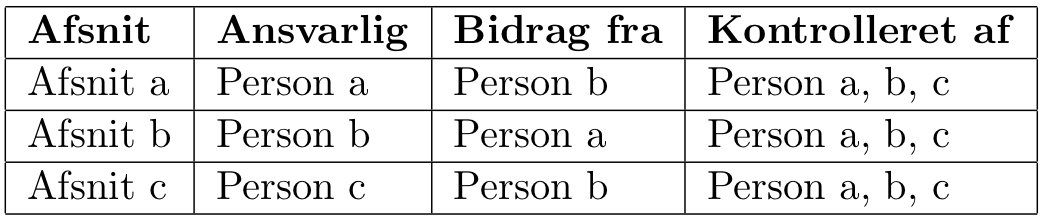
\includegraphics[scale=0.49]{images/kontolskema_bilag_F.png}

                                &           \\ \hline
                                
\textbf{Indledning}     & Projektets rammer og baggrunden for projektet.
Resume af udleverede case.
Problemformulering og afgrænsninger. 
Formål og mål med projektet.
Problemformulering og afgrænsninger. 
\textit{(indledningen må gerne includere materiale direkte fra inceptionsdokumentet, det skal blot have en tydelig reference)}
                                &   +         \\ \hline
                                
\textbf{Faglig vidensgrundlag}  & Begrebsdefinitioner, teori og  fagligt vidensgrundlag.
                                &    +        \\ \hline
                                
\textbf{Metode og planlægning} & \textbf{Metode:} 
Benyttede metoder i projekt (hele projektet).
Kombination af UP og Scrum. Fordele og ulemper
                                &   +         \\ \hline
                                
                            & \textbf{Planlægning:} 
Plan for elaborationsfasen og de enkelte iterationer. Prioritering af krav i planlægningen.
Det faktiske udviklingsarbejde. Faserne, iterationerne og det faktiske  arbejde i dem?
Scrum: backlogs, roller, begivenheder, scrum-buts.
                                &    +        \\ \hline

\textbf{Hovedtekst}
(skal indeholde resultater både fra iteration 1 og fra iteration 2)
    & \textbf{Overordnede krav:}
    Opdateret resume af overordnede krav fra inceptionsdokument inklusive overordnet brugsmønsterdiagram og oversigt over supplerende krav.
                                    &   +         \\ \hline
    & \textbf{Detaljerede krav:}
    Detaljeret brugsmønsterdiagram (hvis relevant).
    Detaljerede brugsmønsterbeskrivelser.
    Detaljerede beskrivelser af supplerende krav, fx organiseret efter FURPS+.
                                        &   +         \\ \hline
    & \textbf{Analyse:} 
    Overvejelser, beslutninger og resultater vedr. analysemodellen, inklusive både den statiske og den dynamiske side af analysemodel. 
                                        &    +       \\ \hline
    & \textbf{Design:}
    Overvejelser, beslutninger og resultater vedr. Softwarearkitektur og detaljeret design, herunder design af persistens. 
                                        &   +        \\ \hline
    & \textbf{Databasedesign:}
    Overvejelser, beslutninger og resultater vedr. tabeldesign og SQL-forespørgsler.
                                        &     +      \\ \hline
    & \textbf{Implementering:}
    Overvejelser, beslutninger og resultater vedr.  konvertering fra design til kode illustreret gennem udvalgte centrale eksempler, samt andre vigtige implementeringsbeslutninger. 
    Implementering af database.
                                        &    +       \\ \hline
    & \textbf{Test:}
    udførte test samt resultatet af dem.
                                        &    +       \\ \hline

\textbf{Diskussion} & Hvad er der opnået og hvad er der ikke opnået i projektet i forhold til det forventede som beskrevet i indledningen. 
Hvad er styrkerne og svaghederne ved resultaterne.
Kunne I have opnået bedre resultater?
                                        &   +        \\ \hline

\textbf{Konklusion} & Opsummering af resultaterne og diskussionen af dem. Svar på problemformuleringen. 
                                        &    +       \\ \hline

\textbf{Perspektivering}   & Er den fundne løsning brugbar i anden sammenhæng?
Hvad bidrager løsningen og den opnåede viden til. 
Fremtidigt arbejde (næste skridt i projektet, hvis I havde mere tid).
                                        &   +        \\ \hline

\textbf{Procesevaluering}   & Processen og gruppens refleksion over processen: Læringsprocessen, teamroller, samarbejdet internt i gruppen og med vejleder, projektarbejdsformen, arbejdsformer, metoder, skriveprocessen, den tidsmæssige styring af projektet,ledelse af projektet, arbejdsfordeling i projektet m.m. 
Hvordan ville I gribe arbejdet an, hvis I skulle starte forfra?
                                        &   +        \\ \hline

\textbf{Referenceliste}   & Litteratur angivet på en anerkendt form. 
(Alle former for litteratur som bøger, artikler og hjemmesider)
Kildehenvisninger i teksten. Materiale som gruppen ikke selv har fremstillet i dette projekt skal være angivet med kilde! 
Alle kildehenvisninger i teksten skal være anført på samme måde. Kildeangivelser på figurer, grafer etc. som projektgruppen ikke selv har frembragt. 
                                        &     +      \\ \hline

\textbf{Bilag}   &
\makecell[l]{
A. Oversigt over kildekode \\
B. Brugervejledning \\
C. Samarbejdsaftale \\
D. Vejlederaftale \\
E. Projektlog \\
F. Udfyldt rapportkontrolskema \\
G. Inceptionsdokument \\
I.  (Andre Bilag) \\
}
                                        &           \\ \hline

\end{longtable}

\begin{longtable}{|p{30mm}|p{90mm}|p{25mm}|}
\hline
\multicolumn{3}{|c|}{\textbf{Rapporttekniske elementer}} \\ \hline

\textbf{Layout} & Er der anvendt samme layout i alle kapitler. 
Er layout overskueligt/harmonisk.
                                        &           \\ \hline

\textbf{Sprog} & Formidler rapporten projektet faglig og sagligt.
Er sproget  neutralt, aktivt, upersonligt, konkret, præcist, kortfattet og korrekt.
(Procesevalueringen må benytte personligt sprog)
                                        &           \\ \hline

\textbf{Sidenummerer-ing} & Er der korrekt og konsistent sidenummerering i rapporten. 
                                        &   ++ \\ \hline

\textbf{Figurer/dia-grammer} & Er alle figurer konsekvent nummererede.
Er der figurtitel og figurtekst til alle figurer.
Er figurtitler og figurtekster dækkende og afklarende.
Er figurerne tydelige og læsbare.
Er figurerne informationsgivende og i den rette sammenhæng.
                                        &    +       \\ \hline

\textbf{Tabeller} & Er alle tabeller konsekvent nummererede.
Er der en forklarende tabeltekst til alle tabeller.
Er alle søjler og rækker forsynet med parametre.
Er der enheder på alle relevante rækker og søjler.
                                        &    +       \\ \hline

\textbf{Sporbarhed af begreber} & Er der en konsekvent brug af samme betegnelse for et givet begreb igennem rapporten. 
                                        &      +     \\ \hline



\end{longtable}

